\documentclass[tikz]{standalone}

\usepackage[utf8]{inputenc}
\usepackage[T1]{fontenc}
\usepackage{cmap}
\usepackage{amsmath}
\usepackage{amssymb}
\usepackage{verbatim}
\usepackage{bm}

\renewcommand{\familydefault}{\sfdefault}
\usepackage[cm]{sfmath}

\usetikzlibrary{bending}
\usetikzlibrary{decorations.pathreplacing}
\usetikzlibrary{decorations.pathmorphing}
\usetikzlibrary{fadings}

\definecolor{cblue}{rgb}{0.396, 0.643, 0.82}
\definecolor{corange}{rgb}{1.0, 0.69, 0.416}
\definecolor{cgreen}{rgb}{0.471, 0.824, 0.471}
\definecolor{cred}{rgb}{1.0, 0.502, 0.502}
\definecolor{cpurple}{rgb}{0.863, 0.78, 0.937}

\begin{document}
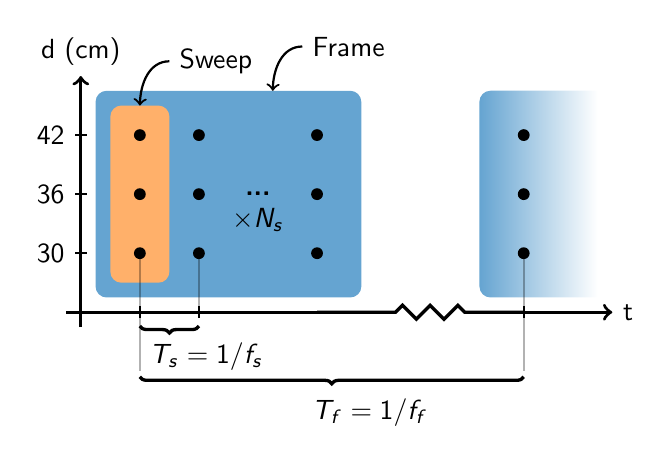
\begin{tikzpicture}[scale=3/4]

% axes
\draw [very thick] (-0.25, 0) -- (4, 0);
\draw [very thick, decoration=straight zigzag, decorate] (4, 0) -- (7.5, 0);
\draw [->, very thick] (7.5, 0) -- (9, 0) node[right]{t};
\draw [->, very thick] (0, -0.25) -- (0, 4) node[above]{d (cm)};

% sweep and frame boxes
\fill [fill=cblue, rounded corners] (0.25, 0.25) rectangle ++(4.5, 3.5);
\fill [fill=corange, rounded corners] (0.5, 0.5) rectangle ++(1, 3);

\fill [fill=cblue, rounded corners, path fading=east] (8.75, 0.25) -- ++(-2, 0) -- ++(0, 3.5) -- ++(2, 0);

% sweep and frame labels
\draw [<-, thick] (1, 3.5) to [out=90, in=180] ++(0.5, 0.75) node [right] {Sweep};
\draw [<-, thick] (3.25, 3.75) to [out=90, in=180] ++(0.5, 0.75) node [right] {Frame};

% points
\foreach \y/\ytext in {0/30, 1/36, 2/42} {
    \foreach \x in {0, 1, 3, 6.5} {
        \fill (\x + 1, \y + 1) circle (1mm);
    }

    % y ticks
    \draw [thick] (0.1, \y + 1) -- ++(-0.2, 0) node [left] {\ytext};
}

% repeat for number of sweeps
\node at (3, 2) {$\bm\ldots$};
\node [below=1.5pt] at (3, 2) {$\times N_s$};

% x ticks
\foreach \x in {1, 2, 7.5} {
    \draw [thick] (\x, 0.1) -- ++(0, -0.2);
}

% x lines
\draw [thick, opacity=0.3] (1, 1) -- (1, -1);
\draw [thick, opacity=0.3] (7.5, 1) -- ++(0, -2);
\draw [thick, opacity=0.3] (2, 1) -- (2, 0);

% x curlys
\draw [very thick, decoration={brace, mirror, raise=5pt}, decorate] (1, 0) -- (2, 0);
\node [right] at (1, -0.75) {$T_s = 1/f_s$};

\draw [very thick, decoration={brace, mirror, raise=2pt}, decorate] (1, -1.0) -- (7.5, -1.0);
\node [right] at (3.75, -1.7) {$T_f = 1/f_f$};

\end{tikzpicture}
\end{document}
